
% Default to the notebook output style

    


% Inherit from the specified cell style.




    
\documentclass[11pt]{article}

    
    
    \usepackage[T1]{fontenc}
    % Nicer default font (+ math font) than Computer Modern for most use cases
    \usepackage{mathpazo}

    % Basic figure setup, for now with no caption control since it's done
    % automatically by Pandoc (which extracts ![](path) syntax from Markdown).
    \usepackage{graphicx}
    % We will generate all images so they have a width \maxwidth. This means
    % that they will get their normal width if they fit onto the page, but
    % are scaled down if they would overflow the margins.
    \makeatletter
    \def\maxwidth{\ifdim\Gin@nat@width>\linewidth\linewidth
    \else\Gin@nat@width\fi}
    \makeatother
    \let\Oldincludegraphics\includegraphics
    % Set max figure width to be 80% of text width, for now hardcoded.
    \renewcommand{\includegraphics}[1]{\Oldincludegraphics[width=.8\maxwidth]{#1}}
    % Ensure that by default, figures have no caption (until we provide a
    % proper Figure object with a Caption API and a way to capture that
    % in the conversion process - todo).
    \usepackage{caption}
    \DeclareCaptionLabelFormat{nolabel}{}
    \captionsetup{labelformat=nolabel}

    \usepackage{adjustbox} % Used to constrain images to a maximum size 
    \usepackage{xcolor} % Allow colors to be defined
    \usepackage{enumerate} % Needed for markdown enumerations to work
    \usepackage{geometry} % Used to adjust the document margins
    \usepackage{amsmath} % Equations
    \usepackage{amssymb} % Equations
    \usepackage{textcomp} % defines textquotesingle
    % Hack from http://tex.stackexchange.com/a/47451/13684:
    \AtBeginDocument{%
        \def\PYZsq{\textquotesingle}% Upright quotes in Pygmentized code
    }
    \usepackage{upquote} % Upright quotes for verbatim code
    \usepackage{eurosym} % defines \euro
    \usepackage[mathletters]{ucs} % Extended unicode (utf-8) support
    \usepackage[utf8x]{inputenc} % Allow utf-8 characters in the tex document
    \usepackage{fancyvrb} % verbatim replacement that allows latex
    \usepackage{grffile} % extends the file name processing of package graphics 
                         % to support a larger range 
    % The hyperref package gives us a pdf with properly built
    % internal navigation ('pdf bookmarks' for the table of contents,
    % internal cross-reference links, web links for URLs, etc.)
    \usepackage{hyperref}
    \usepackage{longtable} % longtable support required by pandoc >1.10
    \usepackage{booktabs}  % table support for pandoc > 1.12.2
    \usepackage[inline]{enumitem} % IRkernel/repr support (it uses the enumerate* environment)
    \usepackage[normalem]{ulem} % ulem is needed to support strikethroughs (\sout)
                                % normalem makes italics be italics, not underlines
    

    
    
    % Colors for the hyperref package
    \definecolor{urlcolor}{rgb}{0,.145,.698}
    \definecolor{linkcolor}{rgb}{.71,0.21,0.01}
    \definecolor{citecolor}{rgb}{.12,.54,.11}

    % ANSI colors
    \definecolor{ansi-black}{HTML}{3E424D}
    \definecolor{ansi-black-intense}{HTML}{282C36}
    \definecolor{ansi-red}{HTML}{E75C58}
    \definecolor{ansi-red-intense}{HTML}{B22B31}
    \definecolor{ansi-green}{HTML}{00A250}
    \definecolor{ansi-green-intense}{HTML}{007427}
    \definecolor{ansi-yellow}{HTML}{DDB62B}
    \definecolor{ansi-yellow-intense}{HTML}{B27D12}
    \definecolor{ansi-blue}{HTML}{208FFB}
    \definecolor{ansi-blue-intense}{HTML}{0065CA}
    \definecolor{ansi-magenta}{HTML}{D160C4}
    \definecolor{ansi-magenta-intense}{HTML}{A03196}
    \definecolor{ansi-cyan}{HTML}{60C6C8}
    \definecolor{ansi-cyan-intense}{HTML}{258F8F}
    \definecolor{ansi-white}{HTML}{C5C1B4}
    \definecolor{ansi-white-intense}{HTML}{A1A6B2}

    % commands and environments needed by pandoc snippets
    % extracted from the output of `pandoc -s`
    \providecommand{\tightlist}{%
      \setlength{\itemsep}{0pt}\setlength{\parskip}{0pt}}
    \DefineVerbatimEnvironment{Highlighting}{Verbatim}{commandchars=\\\{\}}
    % Add ',fontsize=\small' for more characters per line
    \newenvironment{Shaded}{}{}
    \newcommand{\KeywordTok}[1]{\textcolor[rgb]{0.00,0.44,0.13}{\textbf{{#1}}}}
    \newcommand{\DataTypeTok}[1]{\textcolor[rgb]{0.56,0.13,0.00}{{#1}}}
    \newcommand{\DecValTok}[1]{\textcolor[rgb]{0.25,0.63,0.44}{{#1}}}
    \newcommand{\BaseNTok}[1]{\textcolor[rgb]{0.25,0.63,0.44}{{#1}}}
    \newcommand{\FloatTok}[1]{\textcolor[rgb]{0.25,0.63,0.44}{{#1}}}
    \newcommand{\CharTok}[1]{\textcolor[rgb]{0.25,0.44,0.63}{{#1}}}
    \newcommand{\StringTok}[1]{\textcolor[rgb]{0.25,0.44,0.63}{{#1}}}
    \newcommand{\CommentTok}[1]{\textcolor[rgb]{0.38,0.63,0.69}{\textit{{#1}}}}
    \newcommand{\OtherTok}[1]{\textcolor[rgb]{0.00,0.44,0.13}{{#1}}}
    \newcommand{\AlertTok}[1]{\textcolor[rgb]{1.00,0.00,0.00}{\textbf{{#1}}}}
    \newcommand{\FunctionTok}[1]{\textcolor[rgb]{0.02,0.16,0.49}{{#1}}}
    \newcommand{\RegionMarkerTok}[1]{{#1}}
    \newcommand{\ErrorTok}[1]{\textcolor[rgb]{1.00,0.00,0.00}{\textbf{{#1}}}}
    \newcommand{\NormalTok}[1]{{#1}}
    
    % Additional commands for more recent versions of Pandoc
    \newcommand{\ConstantTok}[1]{\textcolor[rgb]{0.53,0.00,0.00}{{#1}}}
    \newcommand{\SpecialCharTok}[1]{\textcolor[rgb]{0.25,0.44,0.63}{{#1}}}
    \newcommand{\VerbatimStringTok}[1]{\textcolor[rgb]{0.25,0.44,0.63}{{#1}}}
    \newcommand{\SpecialStringTok}[1]{\textcolor[rgb]{0.73,0.40,0.53}{{#1}}}
    \newcommand{\ImportTok}[1]{{#1}}
    \newcommand{\DocumentationTok}[1]{\textcolor[rgb]{0.73,0.13,0.13}{\textit{{#1}}}}
    \newcommand{\AnnotationTok}[1]{\textcolor[rgb]{0.38,0.63,0.69}{\textbf{\textit{{#1}}}}}
    \newcommand{\CommentVarTok}[1]{\textcolor[rgb]{0.38,0.63,0.69}{\textbf{\textit{{#1}}}}}
    \newcommand{\VariableTok}[1]{\textcolor[rgb]{0.10,0.09,0.49}{{#1}}}
    \newcommand{\ControlFlowTok}[1]{\textcolor[rgb]{0.00,0.44,0.13}{\textbf{{#1}}}}
    \newcommand{\OperatorTok}[1]{\textcolor[rgb]{0.40,0.40,0.40}{{#1}}}
    \newcommand{\BuiltInTok}[1]{{#1}}
    \newcommand{\ExtensionTok}[1]{{#1}}
    \newcommand{\PreprocessorTok}[1]{\textcolor[rgb]{0.74,0.48,0.00}{{#1}}}
    \newcommand{\AttributeTok}[1]{\textcolor[rgb]{0.49,0.56,0.16}{{#1}}}
    \newcommand{\InformationTok}[1]{\textcolor[rgb]{0.38,0.63,0.69}{\textbf{\textit{{#1}}}}}
    \newcommand{\WarningTok}[1]{\textcolor[rgb]{0.38,0.63,0.69}{\textbf{\textit{{#1}}}}}
    
    
    % Define a nice break command that doesn't care if a line doesn't already
    % exist.
    \def\br{\hspace*{\fill} \\* }
    % Math Jax compatability definitions
    \def\gt{>}
    \def\lt{<}
    % Document parameters
    \title{Doc}
    
    
    

    % Pygments definitions
    
\makeatletter
\def\PY@reset{\let\PY@it=\relax \let\PY@bf=\relax%
    \let\PY@ul=\relax \let\PY@tc=\relax%
    \let\PY@bc=\relax \let\PY@ff=\relax}
\def\PY@tok#1{\csname PY@tok@#1\endcsname}
\def\PY@toks#1+{\ifx\relax#1\empty\else%
    \PY@tok{#1}\expandafter\PY@toks\fi}
\def\PY@do#1{\PY@bc{\PY@tc{\PY@ul{%
    \PY@it{\PY@bf{\PY@ff{#1}}}}}}}
\def\PY#1#2{\PY@reset\PY@toks#1+\relax+\PY@do{#2}}

\expandafter\def\csname PY@tok@w\endcsname{\def\PY@tc##1{\textcolor[rgb]{0.73,0.73,0.73}{##1}}}
\expandafter\def\csname PY@tok@c\endcsname{\let\PY@it=\textit\def\PY@tc##1{\textcolor[rgb]{0.25,0.50,0.50}{##1}}}
\expandafter\def\csname PY@tok@cp\endcsname{\def\PY@tc##1{\textcolor[rgb]{0.74,0.48,0.00}{##1}}}
\expandafter\def\csname PY@tok@k\endcsname{\let\PY@bf=\textbf\def\PY@tc##1{\textcolor[rgb]{0.00,0.50,0.00}{##1}}}
\expandafter\def\csname PY@tok@kp\endcsname{\def\PY@tc##1{\textcolor[rgb]{0.00,0.50,0.00}{##1}}}
\expandafter\def\csname PY@tok@kt\endcsname{\def\PY@tc##1{\textcolor[rgb]{0.69,0.00,0.25}{##1}}}
\expandafter\def\csname PY@tok@o\endcsname{\def\PY@tc##1{\textcolor[rgb]{0.40,0.40,0.40}{##1}}}
\expandafter\def\csname PY@tok@ow\endcsname{\let\PY@bf=\textbf\def\PY@tc##1{\textcolor[rgb]{0.67,0.13,1.00}{##1}}}
\expandafter\def\csname PY@tok@nb\endcsname{\def\PY@tc##1{\textcolor[rgb]{0.00,0.50,0.00}{##1}}}
\expandafter\def\csname PY@tok@nf\endcsname{\def\PY@tc##1{\textcolor[rgb]{0.00,0.00,1.00}{##1}}}
\expandafter\def\csname PY@tok@nc\endcsname{\let\PY@bf=\textbf\def\PY@tc##1{\textcolor[rgb]{0.00,0.00,1.00}{##1}}}
\expandafter\def\csname PY@tok@nn\endcsname{\let\PY@bf=\textbf\def\PY@tc##1{\textcolor[rgb]{0.00,0.00,1.00}{##1}}}
\expandafter\def\csname PY@tok@ne\endcsname{\let\PY@bf=\textbf\def\PY@tc##1{\textcolor[rgb]{0.82,0.25,0.23}{##1}}}
\expandafter\def\csname PY@tok@nv\endcsname{\def\PY@tc##1{\textcolor[rgb]{0.10,0.09,0.49}{##1}}}
\expandafter\def\csname PY@tok@no\endcsname{\def\PY@tc##1{\textcolor[rgb]{0.53,0.00,0.00}{##1}}}
\expandafter\def\csname PY@tok@nl\endcsname{\def\PY@tc##1{\textcolor[rgb]{0.63,0.63,0.00}{##1}}}
\expandafter\def\csname PY@tok@ni\endcsname{\let\PY@bf=\textbf\def\PY@tc##1{\textcolor[rgb]{0.60,0.60,0.60}{##1}}}
\expandafter\def\csname PY@tok@na\endcsname{\def\PY@tc##1{\textcolor[rgb]{0.49,0.56,0.16}{##1}}}
\expandafter\def\csname PY@tok@nt\endcsname{\let\PY@bf=\textbf\def\PY@tc##1{\textcolor[rgb]{0.00,0.50,0.00}{##1}}}
\expandafter\def\csname PY@tok@nd\endcsname{\def\PY@tc##1{\textcolor[rgb]{0.67,0.13,1.00}{##1}}}
\expandafter\def\csname PY@tok@s\endcsname{\def\PY@tc##1{\textcolor[rgb]{0.73,0.13,0.13}{##1}}}
\expandafter\def\csname PY@tok@sd\endcsname{\let\PY@it=\textit\def\PY@tc##1{\textcolor[rgb]{0.73,0.13,0.13}{##1}}}
\expandafter\def\csname PY@tok@si\endcsname{\let\PY@bf=\textbf\def\PY@tc##1{\textcolor[rgb]{0.73,0.40,0.53}{##1}}}
\expandafter\def\csname PY@tok@se\endcsname{\let\PY@bf=\textbf\def\PY@tc##1{\textcolor[rgb]{0.73,0.40,0.13}{##1}}}
\expandafter\def\csname PY@tok@sr\endcsname{\def\PY@tc##1{\textcolor[rgb]{0.73,0.40,0.53}{##1}}}
\expandafter\def\csname PY@tok@ss\endcsname{\def\PY@tc##1{\textcolor[rgb]{0.10,0.09,0.49}{##1}}}
\expandafter\def\csname PY@tok@sx\endcsname{\def\PY@tc##1{\textcolor[rgb]{0.00,0.50,0.00}{##1}}}
\expandafter\def\csname PY@tok@m\endcsname{\def\PY@tc##1{\textcolor[rgb]{0.40,0.40,0.40}{##1}}}
\expandafter\def\csname PY@tok@gh\endcsname{\let\PY@bf=\textbf\def\PY@tc##1{\textcolor[rgb]{0.00,0.00,0.50}{##1}}}
\expandafter\def\csname PY@tok@gu\endcsname{\let\PY@bf=\textbf\def\PY@tc##1{\textcolor[rgb]{0.50,0.00,0.50}{##1}}}
\expandafter\def\csname PY@tok@gd\endcsname{\def\PY@tc##1{\textcolor[rgb]{0.63,0.00,0.00}{##1}}}
\expandafter\def\csname PY@tok@gi\endcsname{\def\PY@tc##1{\textcolor[rgb]{0.00,0.63,0.00}{##1}}}
\expandafter\def\csname PY@tok@gr\endcsname{\def\PY@tc##1{\textcolor[rgb]{1.00,0.00,0.00}{##1}}}
\expandafter\def\csname PY@tok@ge\endcsname{\let\PY@it=\textit}
\expandafter\def\csname PY@tok@gs\endcsname{\let\PY@bf=\textbf}
\expandafter\def\csname PY@tok@gp\endcsname{\let\PY@bf=\textbf\def\PY@tc##1{\textcolor[rgb]{0.00,0.00,0.50}{##1}}}
\expandafter\def\csname PY@tok@go\endcsname{\def\PY@tc##1{\textcolor[rgb]{0.53,0.53,0.53}{##1}}}
\expandafter\def\csname PY@tok@gt\endcsname{\def\PY@tc##1{\textcolor[rgb]{0.00,0.27,0.87}{##1}}}
\expandafter\def\csname PY@tok@err\endcsname{\def\PY@bc##1{\setlength{\fboxsep}{0pt}\fcolorbox[rgb]{1.00,0.00,0.00}{1,1,1}{\strut ##1}}}
\expandafter\def\csname PY@tok@kc\endcsname{\let\PY@bf=\textbf\def\PY@tc##1{\textcolor[rgb]{0.00,0.50,0.00}{##1}}}
\expandafter\def\csname PY@tok@kd\endcsname{\let\PY@bf=\textbf\def\PY@tc##1{\textcolor[rgb]{0.00,0.50,0.00}{##1}}}
\expandafter\def\csname PY@tok@kn\endcsname{\let\PY@bf=\textbf\def\PY@tc##1{\textcolor[rgb]{0.00,0.50,0.00}{##1}}}
\expandafter\def\csname PY@tok@kr\endcsname{\let\PY@bf=\textbf\def\PY@tc##1{\textcolor[rgb]{0.00,0.50,0.00}{##1}}}
\expandafter\def\csname PY@tok@bp\endcsname{\def\PY@tc##1{\textcolor[rgb]{0.00,0.50,0.00}{##1}}}
\expandafter\def\csname PY@tok@fm\endcsname{\def\PY@tc##1{\textcolor[rgb]{0.00,0.00,1.00}{##1}}}
\expandafter\def\csname PY@tok@vc\endcsname{\def\PY@tc##1{\textcolor[rgb]{0.10,0.09,0.49}{##1}}}
\expandafter\def\csname PY@tok@vg\endcsname{\def\PY@tc##1{\textcolor[rgb]{0.10,0.09,0.49}{##1}}}
\expandafter\def\csname PY@tok@vi\endcsname{\def\PY@tc##1{\textcolor[rgb]{0.10,0.09,0.49}{##1}}}
\expandafter\def\csname PY@tok@vm\endcsname{\def\PY@tc##1{\textcolor[rgb]{0.10,0.09,0.49}{##1}}}
\expandafter\def\csname PY@tok@sa\endcsname{\def\PY@tc##1{\textcolor[rgb]{0.73,0.13,0.13}{##1}}}
\expandafter\def\csname PY@tok@sb\endcsname{\def\PY@tc##1{\textcolor[rgb]{0.73,0.13,0.13}{##1}}}
\expandafter\def\csname PY@tok@sc\endcsname{\def\PY@tc##1{\textcolor[rgb]{0.73,0.13,0.13}{##1}}}
\expandafter\def\csname PY@tok@dl\endcsname{\def\PY@tc##1{\textcolor[rgb]{0.73,0.13,0.13}{##1}}}
\expandafter\def\csname PY@tok@s2\endcsname{\def\PY@tc##1{\textcolor[rgb]{0.73,0.13,0.13}{##1}}}
\expandafter\def\csname PY@tok@sh\endcsname{\def\PY@tc##1{\textcolor[rgb]{0.73,0.13,0.13}{##1}}}
\expandafter\def\csname PY@tok@s1\endcsname{\def\PY@tc##1{\textcolor[rgb]{0.73,0.13,0.13}{##1}}}
\expandafter\def\csname PY@tok@mb\endcsname{\def\PY@tc##1{\textcolor[rgb]{0.40,0.40,0.40}{##1}}}
\expandafter\def\csname PY@tok@mf\endcsname{\def\PY@tc##1{\textcolor[rgb]{0.40,0.40,0.40}{##1}}}
\expandafter\def\csname PY@tok@mh\endcsname{\def\PY@tc##1{\textcolor[rgb]{0.40,0.40,0.40}{##1}}}
\expandafter\def\csname PY@tok@mi\endcsname{\def\PY@tc##1{\textcolor[rgb]{0.40,0.40,0.40}{##1}}}
\expandafter\def\csname PY@tok@il\endcsname{\def\PY@tc##1{\textcolor[rgb]{0.40,0.40,0.40}{##1}}}
\expandafter\def\csname PY@tok@mo\endcsname{\def\PY@tc##1{\textcolor[rgb]{0.40,0.40,0.40}{##1}}}
\expandafter\def\csname PY@tok@ch\endcsname{\let\PY@it=\textit\def\PY@tc##1{\textcolor[rgb]{0.25,0.50,0.50}{##1}}}
\expandafter\def\csname PY@tok@cm\endcsname{\let\PY@it=\textit\def\PY@tc##1{\textcolor[rgb]{0.25,0.50,0.50}{##1}}}
\expandafter\def\csname PY@tok@cpf\endcsname{\let\PY@it=\textit\def\PY@tc##1{\textcolor[rgb]{0.25,0.50,0.50}{##1}}}
\expandafter\def\csname PY@tok@c1\endcsname{\let\PY@it=\textit\def\PY@tc##1{\textcolor[rgb]{0.25,0.50,0.50}{##1}}}
\expandafter\def\csname PY@tok@cs\endcsname{\let\PY@it=\textit\def\PY@tc##1{\textcolor[rgb]{0.25,0.50,0.50}{##1}}}

\def\PYZbs{\char`\\}
\def\PYZus{\char`\_}
\def\PYZob{\char`\{}
\def\PYZcb{\char`\}}
\def\PYZca{\char`\^}
\def\PYZam{\char`\&}
\def\PYZlt{\char`\<}
\def\PYZgt{\char`\>}
\def\PYZsh{\char`\#}
\def\PYZpc{\char`\%}
\def\PYZdl{\char`\$}
\def\PYZhy{\char`\-}
\def\PYZsq{\char`\'}
\def\PYZdq{\char`\"}
\def\PYZti{\char`\~}
% for compatibility with earlier versions
\def\PYZat{@}
\def\PYZlb{[}
\def\PYZrb{]}
\makeatother


    % Exact colors from NB
    \definecolor{incolor}{rgb}{0.0, 0.0, 0.5}
    \definecolor{outcolor}{rgb}{0.545, 0.0, 0.0}



    
    % Prevent overflowing lines due to hard-to-break entities
    \sloppy 
    % Setup hyperref package
    \hypersetup{
      breaklinks=true,  % so long urls are correctly broken across lines
      colorlinks=true,
      urlcolor=urlcolor,
      linkcolor=linkcolor,
      citecolor=citecolor,
      }
    % Slightly bigger margins than the latex defaults
    
    \geometry{verbose,tmargin=1in,bmargin=1in,lmargin=1in,rmargin=1in}
    
    

    \begin{document}
    
    
    \maketitle
    
    

    
    The Course of Computational Chemisty; Peking University

\begin{center}\rule{0.5\linewidth}{\linethickness}\end{center}

第五次作业------量子计算化学程序说明 Tutorial of Quantum Chemistry
Programing - ver.01

 \textgreater{} 注:
本程序说明最初使用Jupyter完成(ipynb格式),保留并转化成诸多格式如markdown,
tex, pdf,
html。但转化中会出现一些问题比如latex公式显示的问题,以及排版的问题。这里统一建议使用html或ipynb格式阅读本说明。

    \subsection{0.成员与分工}\label{ux6210ux5458ux4e0eux5206ux5de5}

\subparagraph{小组成员: 贺麒霖, 资治, 刘昊明, 滕达, 乔卓然,
贺鑫}\label{ux5c0fux7ec4ux6210ux5458-ux8d3aux9e92ux9716-ux8d44ux6cbb-ux5218ux660aux660e-ux6ed5ux8fbe-ux4e54ux5353ux7136-ux8d3aux946b}

程序部分:由 资治,腾达、乔卓然、贺鑫负责完成\\
文档部分: 由 贺麒霖、刘昊明负责完成\\
分工不是绝对固定,有相互穿插。\\
\#\#\#\#\# 本程序是小组合作的在github私人项目
https://github.com/Utenaq/2018QC-Project-Ab-initio-wavefunction-program,
你也可以找到一个公共版本 https://github.com/XShinHe/Heisenberg,
两者初期是一致的,前者由乔卓然负责,后者由贺鑫负责。

\begin{center}\rule{0.5\linewidth}{\linethickness}\end{center}

    \subsection{1.编译和使用方法}\label{ux7f16ux8bd1ux548cux4f7fux7528ux65b9ux6cd5}

\subsubsection{编译方法}\label{ux7f16ux8bd1ux65b9ux6cd5}

在主目录或\texttt{./src}子目录下,使用\texttt{make}命令进行编译,需要g++支持。

\subsubsection{使用方法}\label{ux4f7fux7528ux65b9ux6cd5}

\begin{longtable}[]{@{}lll@{}}
\toprule
参数 & 内容 & 补充\tabularnewline
\midrule
\endhead
\texttt{main\ -h} & 获得使用帮助 &\tabularnewline
\texttt{main\ -d} & 进行默认的测试计算 (计算HeH+分子) &
测试文件位于\texttt{../test}目录\tabularnewline
\texttt{main\ -f\ {[}file.gjf{]}} & 进行其他测试文件的测试 &
测试文件位于\texttt{../test}目录,
必须使用\texttt{.gjf}文件格式\tabularnewline
\bottomrule
\end{longtable}

可选的的测试文件位于\texttt{../test}下,包括\textbf{H.gjf},
\textbf{He.gjf}, \textbf{H2.gjf}, \textbf{HeH.gjf}, \textbf{H4.gjf},
\textbf{CH4.gjf}.\\
使用的示例如\texttt{main\ -f\ ../test/H2.gjf}.

    \subsection{2.建模的类的定义的说明}\label{ux5efaux6a21ux7684ux7c7bux7684ux5b9aux4e49ux7684ux8bf4ux660e}

从输入文件到构建计算的基组矩阵空间,使用了如下的建模结构 :

\textbf{以下类来自于basic\_Global.h文件}

\textbf{Point}

\begin{quote}
属性

\begin{longtable}[]{@{}lll@{}}
\toprule
名称 & 数据类型 & 含义\tabularnewline
\midrule
\endhead
x & int32 & 位置参数\tabularnewline
y & int32r & 位置参数\tabularnewline
z & int32 & 位置参数\tabularnewline
name & string & 代表一个点的名字, 抽象属性\tabularnewline
\bottomrule
\end{longtable}

方法

\begin{longtable}[]{@{}llll@{}}
\toprule
名称 & 接受参数 & 返回类型 & 含义\tabularnewline
\midrule
\endhead
norm & x, y, z & double & 求Point坐标平方和的均方根\tabularnewline
norm2 & x, y, z & double & 求Point坐标的平方和\tabularnewline
ref\_Point & PointA & Point &
求Point与参考点A的坐标差值所得到的新Point\tabularnewline
ref\_norm & PointA & double & 求ref\_Point的norm值\tabularnewline
ref\_norm2 & PointA & double & 求ref\_Point的norm2值\tabularnewline
operator+ & PointA & Point &
定义两个Point的加法运算,所得新Point的坐标为它们的x,y,z坐标分别相加\tabularnewline
operator- & PointA & Point &
定义两个Point的减法运算,所得新Point的坐标为它们的x,y,z坐标分别相减\tabularnewline
operator* & double & Point &
定义Point和一个数值的乘法运算,所得新Point的坐标为原x,y,z坐标分别乘上接受的常数\tabularnewline
operator/ & double & Point &
定义Point和一个数值的除法运算,所得新Point的坐标为原x,y,z坐标分别除以接受的常数\tabularnewline
operator* & PointA & double & 求两个Point的内积值\tabularnewline
ostream \& operator\textless{}\textless{} & ostream \&output, Point \&P
& ostream & 输出点具备有的性质\tabularnewline
dist\_AB & Point A, Point B & double & 求A,B两点距离\tabularnewline
dist\_AB2 & Point A, Point B & double &
求A,B两点距离的平方\tabularnewline
\bottomrule
\end{longtable}
\end{quote}

\textbf{Orbital} (继承自Point)

\begin{quote}
额外属性

\begin{longtable}[]{@{}lll@{}}
\toprule
名称 & 数据类型 & 含义\tabularnewline
\midrule
\endhead
L & int & 高斯函数x方向的角动量参数\tabularnewline
M & int & 高斯函数y方向的角动量参数\tabularnewline
N & int & 高斯函数z方向的角动量参数\tabularnewline
alpha & double & 高斯函数的alpha\tabularnewline
\bottomrule
\end{longtable}

额外方法

\begin{longtable}[]{@{}llll@{}}
\toprule
名称 & 接受参数 & 返回类型 & 含义\tabularnewline
\midrule
\endhead
set\_Alpha & double & int & 设置轨道的alpha值\tabularnewline
set\_LMN & int ll,mm,nn & int & 设置轨道的l,m,n的值\tabularnewline
set\_XYZ & double xx,yy,zz & int & 设置轨道的x,y,z的值\tabularnewline
set\_XYZ & Point P & int &
将某一点的坐标作为轨道的三维空间坐标\tabularnewline
get\_Point & / & Point &
获取Orbital在Point类上的性质,并将其储存在一个新的点中\tabularnewline
get\_LMN & int ll,mm,nn & int & 获取某一个高斯函数的l,m,n\tabularnewline
get\_XYZ & double xx,yy,zz & int &
获取Orbital的三维空间坐标\tabularnewline
conv\_Aunit & / & int & 将轨道的空间坐标转化为原子单位\tabularnewline
normGTO & / & double & 计算高斯函数的归一化系数\tabularnewline
normGTP & double a & double &
计算高斯函数归一到a时的归一化系数\tabularnewline
\bottomrule
\end{longtable}
\end{quote}

\textbf{Orbital\_cgto} (继承自Orbital)

\begin{quote}
额外属性

\begin{longtable}[]{@{}lll@{}}
\toprule
名称 & 数据类型 & 含义\tabularnewline
\midrule
\endhead
cn & int & cgto中的高斯函数个数\tabularnewline
coeffs & double & 高斯函数前的收缩系数\tabularnewline
alpha & double & 高斯函数的alpha值\tabularnewline
gtos & Orbital & cgto中的高斯函数\tabularnewline
\bottomrule
\end{longtable}

额外方法

\begin{longtable}[]{@{}llll@{}}
\toprule
名称 & 接受参数 & 返回类型 & 含义\tabularnewline
\midrule
\endhead
set\_Cgto & int num & int &
设置Cgto中高斯函数的数量,并建立列表以存储高斯函数\tabularnewline
get\_CA & idx,cc,aa & int &
读取Cgto中编号为第idx个高斯函数的收缩系数和alpha值\tabularnewline
set\_LMN & ll,mm,nn & int &
设置Cgto中每个高斯函数的L,M,N值\tabularnewline
set\_XYZ & xx,yy,zz & int &
设置Cgto中每个高斯函数的x,y,z值\tabularnewline
set\_XYZ & Point P & int &
利用点P的坐标设置Cgto中每个高斯函数的x,y,z值\tabularnewline
conv\_AUnit & / & int & 将坐标转化为原子单位\tabularnewline
get\_Bohr & / & int & 返回高斯函数角动量的和\tabularnewline
normGTO & int k & double &
返回cgto的第k个高斯函数的归一化系数\tabularnewline
\bottomrule
\end{longtable}
\end{quote}

\textbf{Atom} (继承自Point)

\begin{quote}
额外属性

\begin{longtable}[]{@{}lll@{}}
\toprule
名称 & 数据类型 & 含义\tabularnewline
\midrule
\endhead
znum & int & 原子序数\tabularnewline
mass & double & 原子质量\tabularnewline
ncgto & int & 描述该原子的cgto的数量\tabularnewline
cgto & Orbital\_cgto & contracted GTO\tabularnewline
perd & int & 原子所处的周期\tabularnewline
fmly & int & 原子所处的族\tabularnewline
indx & int & 在几何构型中的编号\tabularnewline
frag & int & 所属片段的编号\tabularnewline
\bottomrule
\end{longtable}

额外方法

\begin{longtable}[]{@{}llll@{}}
\toprule
\begin{minipage}[b]{0.11\columnwidth}\raggedright\strut
名称\strut
\end{minipage} & \begin{minipage}[b]{0.28\columnwidth}\raggedright\strut
接受参数\strut
\end{minipage} & \begin{minipage}[b]{0.06\columnwidth}\raggedright\strut
返回类型\strut
\end{minipage} & \begin{minipage}[b]{0.43\columnwidth}\raggedright\strut
含义\strut
\end{minipage}\tabularnewline
\midrule
\endhead
\begin{minipage}[t]{0.11\columnwidth}\raggedright\strut
get\_Point\strut
\end{minipage} & \begin{minipage}[t]{0.28\columnwidth}\raggedright\strut
/\strut
\end{minipage} & \begin{minipage}[t]{0.06\columnwidth}\raggedright\strut
Point\strut
\end{minipage} & \begin{minipage}[t]{0.43\columnwidth}\raggedright\strut
返回原子具备的点的性质\strut
\end{minipage}\tabularnewline
\begin{minipage}[t]{0.11\columnwidth}\raggedright\strut
get\_Point\strut
\end{minipage} & \begin{minipage}[t]{0.28\columnwidth}\raggedright\strut
Point \&P\strut
\end{minipage} & \begin{minipage}[t]{0.06\columnwidth}\raggedright\strut
int\strut
\end{minipage} & \begin{minipage}[t]{0.43\columnwidth}\raggedright\strut
返回原子具备的点的性质\strut
\end{minipage}\tabularnewline
\begin{minipage}[t]{0.11\columnwidth}\raggedright\strut
read\_Atom\strut
\end{minipage} & \begin{minipage}[t]{0.28\columnwidth}\raggedright\strut
string line\strut
\end{minipage} & \begin{minipage}[t]{0.06\columnwidth}\raggedright\strut
int\strut
\end{minipage} & \begin{minipage}[t]{0.43\columnwidth}\raggedright\strut
从一个字符串中读取原子的名称和位置\strut
\end{minipage}\tabularnewline
\begin{minipage}[t]{0.11\columnwidth}\raggedright\strut
link\_Info\strut
\end{minipage} & \begin{minipage}[t]{0.28\columnwidth}\raggedright\strut
string my\_name\strut
\end{minipage} & \begin{minipage}[t]{0.06\columnwidth}\raggedright\strut
int\strut
\end{minipage} & \begin{minipage}[t]{0.43\columnwidth}\raggedright\strut
根据名称找到对应原子的核电荷数、质量、周期和族\strut
\end{minipage}\tabularnewline
\begin{minipage}[t]{0.11\columnwidth}\raggedright\strut
set\_Basis\strut
\end{minipage} & \begin{minipage}[t]{0.28\columnwidth}\raggedright\strut
string my\_bname,int mysplit, int mynumcs{[}{]}, int myidxcs{[}{]}\strut
\end{minipage} & \begin{minipage}[t]{0.06\columnwidth}\raggedright\strut
int\strut
\end{minipage} & \begin{minipage}[t]{0.43\columnwidth}\raggedright\strut
从基组文件中找到所选原子的高斯基函数的总操作安排,会调用到之后定义的函数\strut
\end{minipage}\tabularnewline
\begin{minipage}[t]{0.11\columnwidth}\raggedright\strut
set\_Basisspace\strut
\end{minipage} & \begin{minipage}[t]{0.28\columnwidth}\raggedright\strut
int split, int numcs{[}{]}, int idxcs{[}{]}\strut
\end{minipage} & \begin{minipage}[t]{0.06\columnwidth}\raggedright\strut
int\strut
\end{minipage} & \begin{minipage}[t]{0.43\columnwidth}\raggedright\strut
根据所给基组的种类首先生成储存空间以存放基函数\strut
\end{minipage}\tabularnewline
\begin{minipage}[t]{0.11\columnwidth}\raggedright\strut
read\_Basis\strut
\end{minipage} & \begin{minipage}[t]{0.28\columnwidth}\raggedright\strut
fstream\& input\strut
\end{minipage} & \begin{minipage}[t]{0.06\columnwidth}\raggedright\strut
int\strut
\end{minipage} & \begin{minipage}[t]{0.43\columnwidth}\raggedright\strut
读取基组文件中收缩系数和alpha信息\strut
\end{minipage}\tabularnewline
\begin{minipage}[t]{0.11\columnwidth}\raggedright\strut
conv\_AUnit\strut
\end{minipage} & \begin{minipage}[t]{0.28\columnwidth}\raggedright\strut
/\strut
\end{minipage} & \begin{minipage}[t]{0.06\columnwidth}\raggedright\strut
int\strut
\end{minipage} & \begin{minipage}[t]{0.43\columnwidth}\raggedright\strut
将Atom的x,y,z值转化为原子单位\strut
\end{minipage}\tabularnewline
\begin{minipage}[t]{0.11\columnwidth}\raggedright\strut
operator\textless{}\textless{}\strut
\end{minipage} & \begin{minipage}[t]{0.28\columnwidth}\raggedright\strut
stream \&output, Atom \&At\strut
\end{minipage} & \begin{minipage}[t]{0.06\columnwidth}\raggedright\strut
ostream\strut
\end{minipage} & \begin{minipage}[t]{0.43\columnwidth}\raggedright\strut
输出原子的信息\strut
\end{minipage}\tabularnewline
\bottomrule
\end{longtable}
\end{quote}

\textbf{Molecule} (继承自Atom)

\begin{quote}
额外属性

\begin{longtable}[]{@{}lll@{}}
\toprule
名称 & 数据类型 & 含义\tabularnewline
\midrule
\endhead
Natom & int & 分子所含原子个数\tabularnewline
iatom & int & 原子的序号\tabularnewline
atoms & Atom & 分子所含的所有原子\tabularnewline
\bottomrule
\end{longtable}
\end{quote}

\textbf{System} (继承自Molecule)

\begin{quote}
额外属性

\begin{longtable}[]{@{}lll@{}}
\toprule
名称 & 数据类型 & 含义\tabularnewline
\midrule
\endhead
Nmol & int & 系统中分子的个数\tabularnewline
imol & int & 系统中分子的序号\tabularnewline
moles & Molecule{[}{]} & 系统中的所有分子\tabularnewline
Bname & string & 系统所选用基组类型的名称\tabularnewline
Nbasis & int & 系统中cgto的数量\tabularnewline
split & int & 系统中原子价层轨道的劈裂数\tabularnewline
numcs & int{[}{]} & 用于存放系统中基组收缩系数列表\tabularnewline
idxcs & int{[}{]} & 系统中基组收缩系数的逐个加和的列表\tabularnewline
idmap & int{[}{]} & 系统中原子的第一个cgto在列表中的index\tabularnewline
\bottomrule
\end{longtable}

额外方法

\begin{longtable}[]{@{}llll@{}}
\toprule
名称 & 接受参数 & 返回类型 & 含义\tabularnewline
\midrule
\endhead
set\_Natom & int num & int &
设定系统所继承的分子属性,包括原子个数、原子编号和idmap\tabularnewline
read\_Atom & string line & int &
读取输入文件中的原子坐标和原子序号\tabularnewline
set\_Basis & string my\_bname & int &
根据基组名称,得到numcs,idxcs和split的信息\tabularnewline
set\_Map & / & int &
在原子列表和基函数列表之间建立映射关系\tabularnewline
OrbC & int \&idx & Orbital\_cgto & 返回序号为idx的cgto\tabularnewline
count\_Znum & / & int & 返回系统的总核电荷数\tabularnewline
conv\_AUnit & / & int & 转化为原子单位\tabularnewline
solve\_Top & string line & int &
将系统分解为不同的分子或组成部分\tabularnewline
operator\textless{}\textless{} & stream \&output, System \&S & ostream &
输出系统的信息\tabularnewline
operator{[}{]} & int \&idx & Orbital\_cgto &
返回序号为idx的cgto\tabularnewline
\bottomrule
\end{longtable}
\end{quote}

\textbf{以下类来自于basic\_Parser.h文件}

\textbf{Task}

\begin{quote}
属性

\begin{longtable}[]{@{}lll@{}}
\toprule
名称 & 数据类型 & 含义\tabularnewline
\midrule
\endhead
Hiffile & string & 输入文件名称\tabularnewline
Logfile & string & 输出文件名称\tabularnewline
Maxmen & int &\tabularnewline
job & string & 工作任务\tabularnewline
Method & string & 方法\tabularnewline
Basis & string & 基组标题\tabularnewline
Title & string & 标题\tabularnewline
Charge & int & 电荷\tabularnewline
Smuti & int & 自旋多重度\tabularnewline
Natom & int & 原子个数\tabularnewline
Nelec & int & 电子个数\tabularnewline
Nbasis & int & cgto个数\tabularnewline
\bottomrule
\end{longtable}

方法

\begin{longtable}[]{@{}llll@{}}
\toprule
名称 & 接受参数 & 返回类型 & 含义\tabularnewline
\midrule
\endhead
set\_I0 & string Hiffile, string Logfile & int &
选取输入文件与输出文件\tabularnewline
set\_job & string job, string method, string basis & int &
设置工作任务\tabularnewline
read\_Predo & / & int & 从输入文件中读取原子的信息\tabularnewline
read\_Task & / & int & 从输入文件中读取计算内容的信息\tabularnewline
Taskparser & string term & int &
工作类型、方法和基组的分析程序\tabularnewline
operator\textless{}\textless{} & stream \&output, System \&S & ostream &
输出task的信息\tabularnewline
\bottomrule
\end{longtable}
\end{quote}

\textbf{以下类来自于basic\_SCF.h文件}

\textbf{SCFer}

\begin{quote}
属性

\begin{longtable}[]{@{}lll@{}}
\toprule
名称 & 数据类型 & 含义\tabularnewline
\midrule
\endhead
report & ofstream & 以输出方式打开文件\tabularnewline
tasklink & Task & scf调用的task类\tabularnewline
SYSlink & System & scf调用的system类\tabularnewline
scf\_name & string & scf的名称\tabularnewline
nsz & int & 系统中cgto的数量\tabularnewline
nocc & int & 分子轨道占据数\tabularnewline
threshold & double & 判断scf是否收敛的阈值\tabularnewline
do\_loop & bool & 指示自洽场是否继续或跳出\tabularnewline
eigen\_S & MatrixXd & 重叠积分矩阵S\tabularnewline
eigen\_H & MatrixXd & H积分矩阵\tabularnewline
eigen\_G & MatrixXd & G积分矩阵\tabularnewline
eigen\_J & MatrixXd & J积分矩阵\tabularnewline
eigen\_K & MatrixXd & K积分矩阵\tabularnewline
eigen\_ERI & Tensor4D & ERI矩阵\tabularnewline
eigen\_F & MatrixXd & Fock矩阵\tabularnewline
eigen\_C & MatrixXd & 系数矩阵\tabularnewline
eigen\_P & MatrixXd & 密度矩阵\tabularnewline
eigen\_X & MatrixXd & 变换矩阵\tabularnewline
eigen\_Y & MatrixXd & 逆变换矩阵\tabularnewline
eigen\_Fp & MatrixXd & 正则Fock矩阵F`\tabularnewline
eigen\_Cp & MatrixXd & 正则系数矩阵C'\tabularnewline
eigen\_E & VectorXd & Fock'矩阵的本征值\tabularnewline
E & double & 体系总能量\tabularnewline
E\_old & double & 上一次迭代的体系总能量\tabularnewline
eigen\_P\_old & MatrixXd & 上一次迭代的体系密度矩阵\tabularnewline
list & int* & 指示占据分子轨道的索引表\tabularnewline
\bottomrule
\end{longtable}

MatrixXd和Tensor4D类型的变量是一系列的矩阵,进行scf过程时会计算得到它们。下面很多函数不直接接受参数,他们都使用类的\textbf{this}指针。

方法

\begin{longtable}[]{@{}llll@{}}
\toprule
\begin{minipage}[b]{0.15\columnwidth}\raggedright\strut
名称\strut
\end{minipage} & \begin{minipage}[b]{0.14\columnwidth}\raggedright\strut
接受参数\strut
\end{minipage} & \begin{minipage}[b]{0.09\columnwidth}\raggedright\strut
返回类型\strut
\end{minipage} & \begin{minipage}[b]{0.51\columnwidth}\raggedright\strut
含义\strut
\end{minipage}\tabularnewline
\midrule
\endhead
\begin{minipage}[t]{0.15\columnwidth}\raggedright\strut
set\_Threshold\strut
\end{minipage} & \begin{minipage}[t]{0.14\columnwidth}\raggedright\strut
double myeps\strut
\end{minipage} & \begin{minipage}[t]{0.09\columnwidth}\raggedright\strut
int\strut
\end{minipage} & \begin{minipage}[t]{0.51\columnwidth}\raggedright\strut
设置scf阈值\strut
\end{minipage}\tabularnewline
\begin{minipage}[t]{0.15\columnwidth}\raggedright\strut
set\_Space\strut
\end{minipage} & \begin{minipage}[t]{0.14\columnwidth}\raggedright\strut
Task\& T\strut
\end{minipage} & \begin{minipage}[t]{0.09\columnwidth}\raggedright\strut
int\strut
\end{minipage} & \begin{minipage}[t]{0.51\columnwidth}\raggedright\strut
建立scf所需要的存储数据的空间,包括一系列的矩阵\strut
\end{minipage}\tabularnewline
\begin{minipage}[t]{0.15\columnwidth}\raggedright\strut
loop\_SCF\strut
\end{minipage} & \begin{minipage}[t]{0.14\columnwidth}\raggedright\strut
/\strut
\end{minipage} & \begin{minipage}[t]{0.09\columnwidth}\raggedright\strut
int\strut
\end{minipage} & \begin{minipage}[t]{0.51\columnwidth}\raggedright\strut
scf循环\strut
\end{minipage}\tabularnewline
\begin{minipage}[t]{0.15\columnwidth}\raggedright\strut
calc\_SHERI\strut
\end{minipage} & \begin{minipage}[t]{0.14\columnwidth}\raggedright\strut
System \&SYS, MatrixXd \&S, MatrixXd \&H, Tensor4D \&ERI\strut
\end{minipage} & \begin{minipage}[t]{0.09\columnwidth}\raggedright\strut
int\strut
\end{minipage} & \begin{minipage}[t]{0.51\columnwidth}\raggedright\strut
计算所有需要的单电子积分(S and H )和双电子积分(ERI)\strut
\end{minipage}\tabularnewline
\begin{minipage}[t]{0.15\columnwidth}\raggedright\strut
guess\_P\strut
\end{minipage} & \begin{minipage}[t]{0.14\columnwidth}\raggedright\strut
/\strut
\end{minipage} & \begin{minipage}[t]{0.09\columnwidth}\raggedright\strut
int (0)\strut
\end{minipage} & \begin{minipage}[t]{0.51\columnwidth}\raggedright\strut
生成初始猜测矩阵\strut
\end{minipage}\tabularnewline
\begin{minipage}[t]{0.15\columnwidth}\raggedright\strut
calc\_XY\strut
\end{minipage} & \begin{minipage}[t]{0.14\columnwidth}\raggedright\strut
/\strut
\end{minipage} & \begin{minipage}[t]{0.09\columnwidth}\raggedright\strut
int (0)\strut
\end{minipage} & \begin{minipage}[t]{0.51\columnwidth}\raggedright\strut
对角化S并计算S\textsuperscript{(1/2)和S}(-1/2)矩阵\strut
\end{minipage}\tabularnewline
\begin{minipage}[t]{0.15\columnwidth}\raggedright\strut
calc\_Fock\strut
\end{minipage} & \begin{minipage}[t]{0.14\columnwidth}\raggedright\strut
/\strut
\end{minipage} & \begin{minipage}[t]{0.09\columnwidth}\raggedright\strut
int (0)\strut
\end{minipage} & \begin{minipage}[t]{0.51\columnwidth}\raggedright\strut
计算Fock矩阵\strut
\end{minipage}\tabularnewline
\begin{minipage}[t]{0.15\columnwidth}\raggedright\strut
calc\_Cprim\strut
\end{minipage} & \begin{minipage}[t]{0.14\columnwidth}\raggedright\strut
/\strut
\end{minipage} & \begin{minipage}[t]{0.09\columnwidth}\raggedright\strut
int (0)\strut
\end{minipage} & \begin{minipage}[t]{0.51\columnwidth}\raggedright\strut
计算变换矩阵c\strut
\end{minipage}\tabularnewline
\begin{minipage}[t]{0.15\columnwidth}\raggedright\strut
tr\_Cprim2C\strut
\end{minipage} & \begin{minipage}[t]{0.14\columnwidth}\raggedright\strut
/\strut
\end{minipage} & \begin{minipage}[t]{0.09\columnwidth}\raggedright\strut
int (0)\strut
\end{minipage} & \begin{minipage}[t]{0.51\columnwidth}\raggedright\strut
对变换矩阵c求迹\strut
\end{minipage}\tabularnewline
\begin{minipage}[t]{0.15\columnwidth}\raggedright\strut
calc\_PE\strut
\end{minipage} & \begin{minipage}[t]{0.14\columnwidth}\raggedright\strut
/\strut
\end{minipage} & \begin{minipage}[t]{0.09\columnwidth}\raggedright\strut
int (0)\strut
\end{minipage} & \begin{minipage}[t]{0.51\columnwidth}\raggedright\strut
计算总势能\strut
\end{minipage}\tabularnewline
\begin{minipage}[t]{0.15\columnwidth}\raggedright\strut
report\_SCF\strut
\end{minipage} & \begin{minipage}[t]{0.14\columnwidth}\raggedright\strut
/\strut
\end{minipage} & \begin{minipage}[t]{0.09\columnwidth}\raggedright\strut
int (0)\strut
\end{minipage} & \begin{minipage}[t]{0.51\columnwidth}\raggedright\strut
报告SCF结果\strut
\end{minipage}\tabularnewline
\begin{minipage}[t]{0.15\columnwidth}\raggedright\strut
get\_NE\strut
\end{minipage} & \begin{minipage}[t]{0.14\columnwidth}\raggedright\strut
/\strut
\end{minipage} & \begin{minipage}[t]{0.09\columnwidth}\raggedright\strut
double\strut
\end{minipage} & \begin{minipage}[t]{0.51\columnwidth}\raggedright\strut
计算原子核之间的库伦斥力\strut
\end{minipage}\tabularnewline
\begin{minipage}[t]{0.15\columnwidth}\raggedright\strut
check\_Loop\strut
\end{minipage} & \begin{minipage}[t]{0.14\columnwidth}\raggedright\strut
int cnt\strut
\end{minipage} & \begin{minipage}[t]{0.09\columnwidth}\raggedright\strut
int (0)\strut
\end{minipage} & \begin{minipage}[t]{0.51\columnwidth}\raggedright\strut
检验SCF是否收敛\strut
\end{minipage}\tabularnewline
\begin{minipage}[t]{0.15\columnwidth}\raggedright\strut
m\_Diff\strut
\end{minipage} & \begin{minipage}[t]{0.14\columnwidth}\raggedright\strut
MatrixXd \&M, MatrixXd \&N\strut
\end{minipage} & \begin{minipage}[t]{0.09\columnwidth}\raggedright\strut
double\strut
\end{minipage} & \begin{minipage}[t]{0.51\columnwidth}\raggedright\strut
计算初始和新生成的密度矩阵是否收敛\strut
\end{minipage}\tabularnewline
\bottomrule
\end{longtable}
\end{quote}

    \subsection{3.分子积分的处理}\label{ux5206ux5b50ux79efux5206ux7684ux5904ux7406}

最初使用的是栾助教所给的积分函数。后来换成我们自己写的通用的积分,这里详细说明其计算方法。

    \paragraph{PGTO的表达和积分的计算}\label{pgtoux7684ux8868ux8fbeux548cux79efux5206ux7684ux8ba1ux7b97}

\begin{enumerate}
\def\labelenumi{\arabic{enumi}.}
\item
  归一化系数的计算 对于一个一般的PGTO,我们使用记号
  \(\mid aAlmn\rangle=x^l y^m z^n\exp(-a(\vec{r}-\vec{A})^2)\)来表达。\\
  则首先,考虑一个一般的PGTO的归一化系数N:\\
  \[\frac{1}{N^2}=\int x^{2l} y^{2m} z^{2n}\exp(-2a(\vec{r}-\vec{A})^2)
  \] 利用公式:
  \[\int_{-\infty}^{\infty}x^{2n}e^{-\alpha x^2}=\sqrt{\frac{\pi}{\alpha}}\frac{(2n-1)!!}{(2\alpha)^n}\]
  所以:
  \[\frac{1}{N^2}=(\frac{\pi}{2\alpha})^{3/2}\frac{(2l-1)!!(2m-1)!!(2n-1)!!}{(4\alpha)^{l+m+n}}\]
\item
  GTO乘积定理 对于s-s型的乘积:
  \[\exp(-ar_A^2)\exp(-br_B^2)=K\exp(-(a+b)r_P^2)\]
  其中\(K=\exp(-\frac{ab}{a+b}\overline{AB}^2)\),代表高斯相乘后的最大峰高。而点\(r_P\)就是\(r_A\)和\(r_B\)两点对于他们指数的加权平均的结果。
  广义的乘积定理则可以表述为:
  \[(x^ly^mz^naA)(x^{l'}y^{m'}z^{n'}bB)=[x+\overline{PA}_x]^{l}[x+\overline{PB}_x]^{l'}[y+\overline{PA}_y]^{m}[y+\overline{PB}_y]^{m'}[z+\overline{PA}_z]^{n}[z+\overline{PB}_z]^{n'}K\exp(-\frac{ab}{a+b}r_P^2)\]
\item
  重叠积分的计算
  对于一般的重叠积分可以根据GTO乘积定理和高斯积分公式进行计算,得到如下结果:
  \[\langle aAlmn\mid bBl'm'n'\rangle=KI_xI_yI_z\] 其中以x方向为例:
  \[I_x=\sqrt{\frac{\pi}{a+b}}\sum_{i=0}{[\frac{(l+l')}{2}]} f_{2i}[ll'(\overline{PA})_x(\overline{PB})_x]\frac{(2i-1)!!}{[2(a+b)]^i}\]
  其中\(f\)函数是两个二项式展开的乘积:
  \[f_i[ll'(\overline{PA})_x(\overline{PB})_x] = \sum_{\lambda}^{l}\sum_{\mu}^{l'}\delta_{\lambda+\mu,i}
  \begin{pmatrix}{l \\ \lambda}\end{pmatrix} \begin{pmatrix}{l' \\ \mu}\end{pmatrix} 
  \overline{PA})_x^{l-\lambda}(\overline{PB})_x^{l'-\mu}\]
\item
  动能积分的计算
  动能积分涉及到高斯函数的求导,高斯函数的求导还是高斯类型的函数:
  \[\frac{\partial}{\partial x_A} \mid aAlmn \rangle = (lx_A^{-1}-2ax_A) \mid aAlmn \rangle\]
  \[\frac{\partial^2}{\partial x_A^2} \mid aAlmn \rangle = (l(l-1)x_A^{-2}-2a(2l+1)+4a^2x_A^2) \mid aAlmn \rangle \]
  所以不难转换为重叠积分的计算:
  \[I=  \langle aAl_1m_1n_1 \mid -\frac{1}{2}\nabla^2 \mid bBl_2m_2n_2\rangle = I_x + I_y + I_z \]
  其中以x方向为例: \[\begin{eqnarray}
  & I_x &=& \langle aAl_1m_1n_1 \mid -\frac{1}{2}\frac{\partial^2}{\partial x^2} \mid bBl_2m_2n_2\rangle \\
  &&=& -\frac{1}{2}l_2(l_2-1)\langle aAl_1m_1n_1 \mid bB(l_2-2)m_2n_2\rangle +
   b(2l_2+1)\langle aAl_1m_1n_1 \mid bBl_2m_2n_2\rangle -
  2b^2\langle aAl_1m_1n_1 \mid bB(l_2+2)m_2n_2\rangle 
  \end{eqnarray}\]
\item
  电子-核吸引能积分\\
  使用不完全\(\Gamma\)函数\(F_m(\omega)=\int_0^1 \exp(-\omega t^2)t^{2m}dt\)\\
  \(F_m\)的Taylor展开:
  \[F_m(\omega) = e^{-\omega}\sum_{i=0}^{infty}\frac{(2m-1)!!(2\omega)^i}{(2m+2i+1)!!}\]
  也可以使用递推公式:
  \[F_{m+1}(\omega) = \frac{1}{\omega}[(2m+1)F_m(\omega)-\exp(-\omega)]\]
  以及求导性质: \[F'_m(\omega) = - F_{m+1}(\omega)\] 首先看 s-s
  型的V积分,计算器结果就需要用到laplace变换: \[\begin{eqnarray}
  &\langle ar_A \mid \frac{1}{r_C} \mid br_B \rangle = K \int \exp(-(a+b)r_P^2)\frac{1}{r_C}d\tau \\
  &\overset{laplace}{===} K \int \exp(-(a+b)r_P^2) \Big[\pi^{-1/2}\int_0^\infty \exp(-sr_C^2)s^{-1/2}ds \Big]d\tau \\
  &= K\pi^{-1/2} \int\int_0^\infty \exp(-(a+b)r_P^2)\exp(-sr_C^2)s^{-1/2}dsd\tau \\
  &= K_{AB}\pi \int_0^\infty \exp\Big[-\frac{(a+b)s}{a+b+s}\overline{PC}^2\Big]s^{-1/2}(a+b+s)^{-3/2}ds 
  \end{eqnarray}\]\\
  变量代换\(t^2=s/(a+b+s)\),可以讲对s的积分化成不完全\(\Gamma\)函数\(F_0\):
  \[\langle ar_A \mid \frac{1}{r_C} \mid br_B \rangle = K \frac{2\pi}{a+b}F_0[(a+b)\overline{PC}^2]\]
  对于广义的电子和核吸引势能积分,可以讲高阶的Gauss函数通过对核位置的偏导数降阶,如:
  \[G(a,A,l+1,m,n)=\frac{1}{2a}\Big[\frac{\partial}{\partial A_x}G(a,A,l,m,n) + lG(a,A,l-1,m,n)\Big]\]
  \[\hat{1} = \frac{1}{2a}(\frac{\partial}{\partial A_x}\hat{a}_l + \hat{a}_l \hat{l} \hat{a}_l)\]
  \[\begin{eqnarray}
  & \hat{1}_l = \frac{1}{(2a)^l}(\frac{\partial}{\partial A_x}\hat{a}_l + \tilde{l}\hat{a}_l^2)^l
  & = \frac{1}{(2a)^l}\sum_{i=0}^{l}C_l^i(\frac{\partial}{\partial A_x})^i\hat{a}_l^i \tilde{l}^{l-i}\hat{a}_l^{2l-2i} =  \frac{1}{(2a)^l}(\frac{\partial}{\partial A_x})^l
  \end{eqnarray}\]
  其中\(\hat{a}_l\)为x方向角动量的湮灭算符,并却对与l的指标:\(if\,k>l,\, a^k_l=0\),其中\(\tilde{l}^n\mid l\rangle \overset{def}{=} \frac{\Gamma(l)}{\Gamma(l-n)}\mid l\rangle\)\\
  那么对于任意的一个V积分: \[\begin{eqnarray}
  &&\langle ar_Almn \mid \frac{1}{r_C} \mid br_Bl'm'n' \rangle \\
  &&= \frac{1}{(2a)^{l+m+n}}\frac{1}{(2b)^{l'+m'+n'}}
  (\frac{\partial}{\partial A_x})^l(\frac{\partial}{\partial A_y})^m(\frac{\partial}{\partial A_z})^n
  (\frac{\partial}{\partial B_x})^{l'}(\frac{\partial}{\partial B_y})^{m'}(\frac{\partial}{\partial B_z})^{n'}
  \langle ar_Almn \mid \frac{1}{r_C} \mid br_Bl'm'n' \rangle \\
  &&=\frac{1}{(2a)^{l+m+n}}\frac{1}{(2b)^{l'+m'+n'}}
  (\frac{\partial}{\partial A_x})^l(\frac{\partial}{\partial A_y})^m(\frac{\partial}{\partial A_z})^n
  (\frac{\partial}{\partial B_x})^{l'}(\frac{\partial}{\partial B_y})^{m'}(\frac{\partial}{\partial B_z})^{n'}
  \Big[ K \frac{2\pi}{a+b}F_0[(a+b)\overline{PC}^2] \Big]
  \end{eqnarray}\]
  可以展开为6个二项式展开的乘积,剩下的就是我们需要知道K关于核位置的任意阶导数,以及\(F_0\)关于核位置的任意阶导数。\\
  \[\begin{eqnarray}
  &&(\frac{\partial}{\partial A_x})^l(\frac{\partial}{\partial A_y})^m(\frac{\partial}{\partial A_z})^n
  (\frac{\partial}{\partial B_x})^{l'}(\frac{\partial}{\partial B_y})^{m'}(\frac{\partial}{\partial B_z})^{n'}
  K \\
  &&= (-1)^{l'+m'+n'}(\frac{\partial}{\partial A_x})^{l+l'}(\frac{\partial}{\partial A_y})^{m+m'}(\frac{\partial}{\partial A_z})^{n+n'} \exp[-\frac{ab}{a+b}\overline{AB}^2] 
  \end{eqnarray}\] 对比Hermite多项式的定义:
  \[H_n(x)=(-1)^n e^{x^2}\frac{d^n}{dx^n}e^{-x^2} = n!\sum_{m=0}^{[n/2]}\frac{(-1)^m}{m!(n-2m)!2^m}x^{n-2m}\]
  \[\begin{eqnarray}
  Above = (-1)^{l+m+n}H_{l+l'}(\frac{ab}{a+b})^{(l+m+n+l'+m'+n')/2}(\sqrt{\frac{ab}{a+b}}\overline{AB}_x) H_{m+m'}(\sqrt{\frac{ab}{a+b}}\overline{AB}_y) H_{n+n'}(\sqrt{\frac{ab}{a+b}}\overline{AB}_z)\exp[-\frac{ab}{a+b}\overline{AB}^2] 
  \end{eqnarray}\]
  另外一方面,可以发现,\(F'_m(\omega)=- F_{m+1}(\omega)\),忽略m指标的变化,求导规则与\(e^{-x}\)非常相似,而\(\omega=\alpha_{eff}\overline{PC}^2\),这样也同样的道理,可以通过Herimite多项式处理:
  \[\begin{eqnarray}
  &&(\frac{\partial}{\partial A_x})^l(\frac{\partial}{\partial A_y})^m(\frac{\partial}{\partial A_z})^n
  (\frac{\partial}{\partial B_x})^{l'}(\frac{\partial}{\partial B_y})^{m'}(\frac{\partial}{\partial B_z})^{n'}
  F_0[(a+b)\overline{PC}^2] \\
  &&= (\frac{b}{a+b})^{l+m+n}(\frac{a}{a+b})^{l'+m'+n'}(\frac{\partial}{\partial P_x})^{l+l'}(\frac{\partial}{\partial P_y})^{m+m'}(\frac{\partial}{\partial P_z})^{n+n'} F_0[(a+b)\overline{PC}^2] \\
  &&= (-1)^{l+m+n+l'+m'+n'}(\frac{b}{a+b})^{l+m+n}(\frac{a}{a+b})^{l'+m'+n'}(a+b)^{(l+m+n+l'+m'+n')/2} \\
  &&\times \,H_{l+l'}(\sqrt{a+b}\,\overline{PC}_x)H_{m+m'}(\sqrt{a+b}\,\overline{PC}_y)H_{n+n'}(\sqrt{a+b}\,\overline{PC}_z) F_{l+m+n+l'+m'+n'}[(a+b)\overline{PC}^2]
  \end{eqnarray}\]
\item
  电子排斥能积分的计算\\
  s-s型积分,类似的需要通过laplace变换,这里不假解释了,结果为:
  \[I=\frac{2\pi^{5/2}}{(a+b)(c+d)\sqrt{a+b+c+d}} K_{AB} K_{CD} F_0[\frac{(a+b)(c+d)}{(a+b+c+d)}\overline{PQ}^2]\]
  \[K_{AB}=\exp(-\frac{ab}{a+b}\overline{AB}^2)\]
  \[K_{CD}=\exp(-\frac{cd}{c+d}\overline{CD}^2)\]
  广义的ERI积分通过对原子核运动的12个自由度求偏导数,最终可以降到s-s型积分。着同样转化为若干个二项式展开的乘积(准确来说是12个),同样需要知道\(K_{AB}\),\(K_{CD}\),\(F_0[\alpha_{eff}\overline{PQ}^2]\)对于12个方向的任意阶的偏导数。着同样是通过Hermite多形式得到的。与V积分的约化过程相似。
\end{enumerate}

    \paragraph{\texorpdfstring{积分的函数说明
(\textbf{basic\_Integral.h})}{积分的函数说明 (basic\_Integral.h)}}\label{ux79efux5206ux7684ux51fdux6570ux8bf4ux660e-basic_integral.h}

\begin{quote}
\begin{longtable}[]{@{}llll@{}}
\toprule
\begin{minipage}[b]{0.17\columnwidth}\raggedright\strut
函数名称\strut
\end{minipage} & \begin{minipage}[b]{0.37\columnwidth}\raggedright\strut
接受参数\strut
\end{minipage} & \begin{minipage}[b]{0.07\columnwidth}\raggedright\strut
返回类型\strut
\end{minipage} & \begin{minipage}[b]{0.27\columnwidth}\raggedright\strut
计算含义\strut
\end{minipage}\tabularnewline
\midrule
\endhead
\begin{minipage}[t]{0.17\columnwidth}\raggedright\strut
integral\_S\_sstype\strut
\end{minipage} & \begin{minipage}[t]{0.37\columnwidth}\raggedright\strut
Orbital\_cgto\& cgto1, Orbital\_cgto\& cgto2\strut
\end{minipage} & \begin{minipage}[t]{0.07\columnwidth}\raggedright\strut
double\strut
\end{minipage} & \begin{minipage}[t]{0.27\columnwidth}\raggedright\strut
s-s类型cgto的S积分(不完整版,弃用)\strut
\end{minipage}\tabularnewline
\begin{minipage}[t]{0.17\columnwidth}\raggedright\strut
integral\_ERI\_sstype\strut
\end{minipage} & \begin{minipage}[t]{0.37\columnwidth}\raggedright\strut
Orbital\_cgto\& cgto1, Orbital\_cgto\& cgto2, Orbital\_cgto\& cgto3,
Orbital\_cgto\& cgto4\strut
\end{minipage} & \begin{minipage}[t]{0.07\columnwidth}\raggedright\strut
double\strut
\end{minipage} & \begin{minipage}[t]{0.27\columnwidth}\raggedright\strut
s-s类型cgto的ERI积分(不完整版,弃用)\strut
\end{minipage}\tabularnewline
\begin{minipage}[t]{0.17\columnwidth}\raggedright\strut
integral\_T\_sstype\strut
\end{minipage} & \begin{minipage}[t]{0.37\columnwidth}\raggedright\strut
Orbital\_cgto\& cgto1, Orbital\_cgto\& cgto2\strut
\end{minipage} & \begin{minipage}[t]{0.07\columnwidth}\raggedright\strut
double\strut
\end{minipage} & \begin{minipage}[t]{0.27\columnwidth}\raggedright\strut
s-s类型cgto的T积分(不完整版,弃用)\strut
\end{minipage}\tabularnewline
\begin{minipage}[t]{0.17\columnwidth}\raggedright\strut
integral\_V\_sstype\strut
\end{minipage} & \begin{minipage}[t]{0.37\columnwidth}\raggedright\strut
Orbital\_cgto\& cgto1, Orbital\_cgto\& cgto2, Atom\& P\strut
\end{minipage} & \begin{minipage}[t]{0.07\columnwidth}\raggedright\strut
double\strut
\end{minipage} & \begin{minipage}[t]{0.27\columnwidth}\raggedright\strut
s-s类型cgto的V积分(不完整版,弃用)\strut
\end{minipage}\tabularnewline
\begin{minipage}[t]{0.17\columnwidth}\raggedright\strut
binomial\strut
\end{minipage} & \begin{minipage}[t]{0.37\columnwidth}\raggedright\strut
int a, int b\strut
\end{minipage} & \begin{minipage}[t]{0.07\columnwidth}\raggedright\strut
int\strut
\end{minipage} & \begin{minipage}[t]{0.27\columnwidth}\raggedright\strut
返回二项式系数\(C_a^b\)\strut
\end{minipage}\tabularnewline
\begin{minipage}[t]{0.17\columnwidth}\raggedright\strut
factorial\strut
\end{minipage} & \begin{minipage}[t]{0.37\columnwidth}\raggedright\strut
int a\strut
\end{minipage} & \begin{minipage}[t]{0.07\columnwidth}\raggedright\strut
int\strut
\end{minipage} & \begin{minipage}[t]{0.27\columnwidth}\raggedright\strut
返回阶乘\(a!\)\strut
\end{minipage}\tabularnewline
\begin{minipage}[t]{0.17\columnwidth}\raggedright\strut
doublefactorial\strut
\end{minipage} & \begin{minipage}[t]{0.37\columnwidth}\raggedright\strut
int a\strut
\end{minipage} & \begin{minipage}[t]{0.07\columnwidth}\raggedright\strut
int\strut
\end{minipage} & \begin{minipage}[t]{0.27\columnwidth}\raggedright\strut
返回双阶乘\(a!!\)\strut
\end{minipage}\tabularnewline
\begin{minipage}[t]{0.17\columnwidth}\raggedright\strut
Hermite\_normial\strut
\end{minipage} & \begin{minipage}[t]{0.37\columnwidth}\raggedright\strut
double x, int n\strut
\end{minipage} & \begin{minipage}[t]{0.07\columnwidth}\raggedright\strut
double\strut
\end{minipage} & \begin{minipage}[t]{0.27\columnwidth}\raggedright\strut
返回Hermite多项式\(H_n(x)\)\strut
\end{minipage}\tabularnewline
\begin{minipage}[t]{0.17\columnwidth}\raggedright\strut
Kcoeff\strut
\end{minipage} & \begin{minipage}[t]{0.37\columnwidth}\raggedright\strut
Orbital\& orb1, Orbital\& orb2\strut
\end{minipage} & \begin{minipage}[t]{0.07\columnwidth}\raggedright\strut
double\strut
\end{minipage} & \begin{minipage}[t]{0.27\columnwidth}\raggedright\strut
返回\(exp[-(ab/(a+b))\overline{AB}^2]\)\strut
\end{minipage}\tabularnewline
\begin{minipage}[t]{0.17\columnwidth}\raggedright\strut
general\_Kcoeff\strut
\end{minipage} & \begin{minipage}[t]{0.37\columnwidth}\raggedright\strut
Orbital\& orb1, Orbital\& orb2, int d1, int d2, int d3, int d4, int d5,
int d6\strut
\end{minipage} & \begin{minipage}[t]{0.07\columnwidth}\raggedright\strut
double\strut
\end{minipage} & \begin{minipage}[t]{0.27\columnwidth}\raggedright\strut
返回\(K_{AB}\)在6个核自由度上的任意高阶导数\strut
\end{minipage}\tabularnewline
\begin{minipage}[t]{0.17\columnwidth}\raggedright\strut
general\_Kcoeff\_ERI\strut
\end{minipage} & \begin{minipage}[t]{0.37\columnwidth}\raggedright\strut
Orbital\& orb1, Orbital\& orb2, int d1, int d2, int d3, int d4, int d5,
int d6, int d7, int d8, int d9, int d10, int d11, int d12\strut
\end{minipage} & \begin{minipage}[t]{0.07\columnwidth}\raggedright\strut
double\strut
\end{minipage} & \begin{minipage}[t]{0.27\columnwidth}\raggedright\strut
返回两个K函数乘积\(K_{AB}K_{CD}\)在12个核自由度上的任意高阶导数\strut
\end{minipage}\tabularnewline
\begin{minipage}[t]{0.17\columnwidth}\raggedright\strut
Fn\strut
\end{minipage} & \begin{minipage}[t]{0.37\columnwidth}\raggedright\strut
double w, int m\strut
\end{minipage} & \begin{minipage}[t]{0.07\columnwidth}\raggedright\strut
double\strut
\end{minipage} & \begin{minipage}[t]{0.27\columnwidth}\raggedright\strut
返回m阶的不完全Gamma函数\(F_m(w)\)\strut
\end{minipage}\tabularnewline
\begin{minipage}[t]{0.17\columnwidth}\raggedright\strut
Fn\_pade\strut
\end{minipage} & \begin{minipage}[t]{0.37\columnwidth}\raggedright\strut
double w, int m\strut
\end{minipage} & \begin{minipage}[t]{0.07\columnwidth}\raggedright\strut
double\strut
\end{minipage} & \begin{minipage}[t]{0.27\columnwidth}\raggedright\strut
不完全Gamma函数\(F_m(w)\)的一种pade近似方案\strut
\end{minipage}\tabularnewline
\begin{minipage}[t]{0.17\columnwidth}\raggedright\strut
general\_Fn\_V\strut
\end{minipage} & \begin{minipage}[t]{0.37\columnwidth}\raggedright\strut
Orbital\& orb1, Orbital\& orb2, Atom\& PN, int d1, int d2, int d3, int
d4, int d5, int d6\strut
\end{minipage} & \begin{minipage}[t]{0.07\columnwidth}\raggedright\strut
double\strut
\end{minipage} & \begin{minipage}[t]{0.27\columnwidth}\raggedright\strut
返回Fn函数对于6个核自由度上的高阶导数(用于V积分)\strut
\end{minipage}\tabularnewline
\begin{minipage}[t]{0.17\columnwidth}\raggedright\strut
general\_Fn\_ERI\strut
\end{minipage} & \begin{minipage}[t]{0.37\columnwidth}\raggedright\strut
Orbital\& orb1, Orbital\& orb2, Orbital\& orb3, Orbital\& orb4, int d1,
int d2, int d3, int d4, int d5, int d6, int d7, int d8, int d9, int d10,
int d11, int d12\strut
\end{minipage} & \begin{minipage}[t]{0.07\columnwidth}\raggedright\strut
double\strut
\end{minipage} & \begin{minipage}[t]{0.27\columnwidth}\raggedright\strut
返回Fn函数对于12个核自由度上的高阶导数(用于ERI积分)\strut
\end{minipage}\tabularnewline
\begin{minipage}[t]{0.17\columnwidth}\raggedright\strut
IntecGTO\_S\strut
\end{minipage} & \begin{minipage}[t]{0.37\columnwidth}\raggedright\strut
Orbital\_cgto\& cgto1, Orbital\_cgto\& cgto2\strut
\end{minipage} & \begin{minipage}[t]{0.07\columnwidth}\raggedright\strut
double\strut
\end{minipage} & \begin{minipage}[t]{0.27\columnwidth}\raggedright\strut
广义类型的cgto的S积分\strut
\end{minipage}\tabularnewline
\begin{minipage}[t]{0.17\columnwidth}\raggedright\strut
InteGTO\_S\strut
\end{minipage} & \begin{minipage}[t]{0.37\columnwidth}\raggedright\strut
Orbital\& orb1, Orbital\& orb2\strut
\end{minipage} & \begin{minipage}[t]{0.07\columnwidth}\raggedright\strut
double\strut
\end{minipage} & \begin{minipage}[t]{0.27\columnwidth}\raggedright\strut
广义类型的gto的S积分\strut
\end{minipage}\tabularnewline
\begin{minipage}[t]{0.17\columnwidth}\raggedright\strut
IScoeff\strut
\end{minipage} & \begin{minipage}[t]{0.37\columnwidth}\raggedright\strut
Orbital\& orb1, Orbital\& orb2, char flag\strut
\end{minipage} & \begin{minipage}[t]{0.07\columnwidth}\raggedright\strut
double\strut
\end{minipage} & \begin{minipage}[t]{0.27\columnwidth}\raggedright\strut
广义类型的gto的S积分一维分量\strut
\end{minipage}\tabularnewline
\begin{minipage}[t]{0.17\columnwidth}\raggedright\strut
IntecGTO\_T\strut
\end{minipage} & \begin{minipage}[t]{0.37\columnwidth}\raggedright\strut
Orbital\_cgto\& cgto1, Orbital\_cgto\& cgto2\strut
\end{minipage} & \begin{minipage}[t]{0.07\columnwidth}\raggedright\strut
double\strut
\end{minipage} & \begin{minipage}[t]{0.27\columnwidth}\raggedright\strut
广义类型的cgto的T积分\strut
\end{minipage}\tabularnewline
\begin{minipage}[t]{0.17\columnwidth}\raggedright\strut
InteGTO\_T\strut
\end{minipage} & \begin{minipage}[t]{0.37\columnwidth}\raggedright\strut
Orbital\& orb1, Orbital\& orb2\strut
\end{minipage} & \begin{minipage}[t]{0.07\columnwidth}\raggedright\strut
double\strut
\end{minipage} & \begin{minipage}[t]{0.27\columnwidth}\raggedright\strut
广义类型的gto的T积分\strut
\end{minipage}\tabularnewline
\begin{minipage}[t]{0.17\columnwidth}\raggedright\strut
IntecGTO\_V\strut
\end{minipage} & \begin{minipage}[t]{0.37\columnwidth}\raggedright\strut
Orbital\_cgto\& cgto1, Orbital\_cgto\& cgto2, Atom\& PN\strut
\end{minipage} & \begin{minipage}[t]{0.07\columnwidth}\raggedright\strut
double\strut
\end{minipage} & \begin{minipage}[t]{0.27\columnwidth}\raggedright\strut
广义类型cgto的V积分\strut
\end{minipage}\tabularnewline
\begin{minipage}[t]{0.17\columnwidth}\raggedright\strut
general\_InteGTO\_V\strut
\end{minipage} & \begin{minipage}[t]{0.37\columnwidth}\raggedright\strut
Orbital\& orb1, Orbital\& orb2, Atom\& PN, int f1, int f2, int f3, int
f4, int f5, int f6, int d1, int d2, int d3, int d4, int d5, int d6\strut
\end{minipage} & \begin{minipage}[t]{0.07\columnwidth}\raggedright\strut
double\strut
\end{minipage} & \begin{minipage}[t]{0.27\columnwidth}\raggedright\strut
广义类型gto的V积分(递推法)\strut
\end{minipage}\tabularnewline
\begin{minipage}[t]{0.17\columnwidth}\raggedright\strut
IntecGTO\_ERI\strut
\end{minipage} & \begin{minipage}[t]{0.37\columnwidth}\raggedright\strut
Orbital\_cgto\& cgto1, Orbital\_cgto\& cgto2, Orbital\_cgto\& cgto3,
Orbital\_cgto\& cgto4\strut
\end{minipage} & \begin{minipage}[t]{0.07\columnwidth}\raggedright\strut
double\strut
\end{minipage} & \begin{minipage}[t]{0.27\columnwidth}\raggedright\strut
广义类型cgto的ERI积分\strut
\end{minipage}\tabularnewline
\begin{minipage}[t]{0.17\columnwidth}\raggedright\strut
general\_InteGTO\_ERI\strut
\end{minipage} & \begin{minipage}[t]{0.37\columnwidth}\raggedright\strut
Orbital\& orb1, Orbital\& orb2, Orbital\& orb3, Orbital\& orb4, int f1,
int f2, int f3, int f4, int f5, int f6, int f7, int f8, int f9, int f10,
int f11, int f12, int d1, int d2, int d3, int d4, int d5, int d6, int
d7, int d8, int d9, int d10, int d11, int d12\strut
\end{minipage} & \begin{minipage}[t]{0.07\columnwidth}\raggedright\strut
double\strut
\end{minipage} & \begin{minipage}[t]{0.27\columnwidth}\raggedright\strut
广义类型gto的ERI积分(递推法)\strut
\end{minipage}\tabularnewline
\bottomrule
\end{longtable}
\end{quote}

    \subsection{4.自洽场计算的流程}\label{ux81eaux6d3dux573aux8ba1ux7b97ux7684ux6d41ux7a0b}

    \paragraph{函数说明}\label{ux51fdux6570ux8bf4ux660e}

参见2中的SCFer类。 \#\#\#\# 流程\\
1. \textbf{main} 函数从命令行接收参数,传给解释器
\textbf{basic\_Parser.h}
(也即构建了一个\textbf{Task}对象,并初始化Task).\\
2.
解释器读入输入文件,构造体系、原子、收缩GTO、GTO的信息,并且通过设定的基组,从\texttt{../basis}文件目录读入需要的CGTO参数.
3. 构造一个\textbf{SCFer}对象,由解释器Pasrer将Task对象传给SCFer.
SCFer根据体系的参数确定创建矩阵的大小. 4.
SCFer进入loop\_SCF程序,首先是调用一系列积分函数(\texttt{./basic\_Integral.h}),计算S、H、ERI矩阵等.
并对重叠矩阵对称正交化得到变换矩阵X和其逆矩阵Y. 5.
通过讲H假定成Fock矩阵,预先做一轮SCF,可以得到初始的猜测的密度矩阵P. 6.
通过密度矩阵P、H矩阵、G矩阵计算Fock矩阵F,并使用变换矩阵X变换到F'. 7.
解F'矩阵的本征值问题,得到解本征值e和本征矢空间C',并通过变化矩阵X变换到分子轨道系数矩阵C.
8. 计算确定分子轨道占据,进一步确定总能量E、密度矩阵P. 9.
比较得到的总能量E和密度矩阵P是否与上一步的一致,如果一致则跳出自洽场迭代,否则重复自洽场迭代.

    \subsection{5.
对称性的应用(暂无)}\label{ux5bf9ux79f0ux6027ux7684ux5e94ux7528ux6682ux65e0}

    \subsection{6.测试与结果}\label{ux6d4bux8bd5ux4e0eux7ed3ux679c}

进行测试如下(测试命令参看编译与使用)

\begin{longtable}[]{@{}llll@{}}
\toprule
测试体系 & 结果 {[}au{]} & Gauss09对比{[}au{]} & 结论\tabularnewline
\midrule
\endhead
H & -0.42244193 & -0.4982329 & 不能解决open-shell问题\tabularnewline
He & -2.85516043 & -2.8551604 & 一 致\tabularnewline
H2 & -1.11003090 & -1.1100309 & 一致\tabularnewline
HeH+ & -2.89478689 & -2.8947869 & 一致\tabularnewline
H4 & -1.80246920 & -1.7251712 & 不一致\tabularnewline
CH4 & 震荡问题 & -39.9119255 & 不一致\tabularnewline
\bottomrule
\end{longtable}

    \begin{figure}
\centering
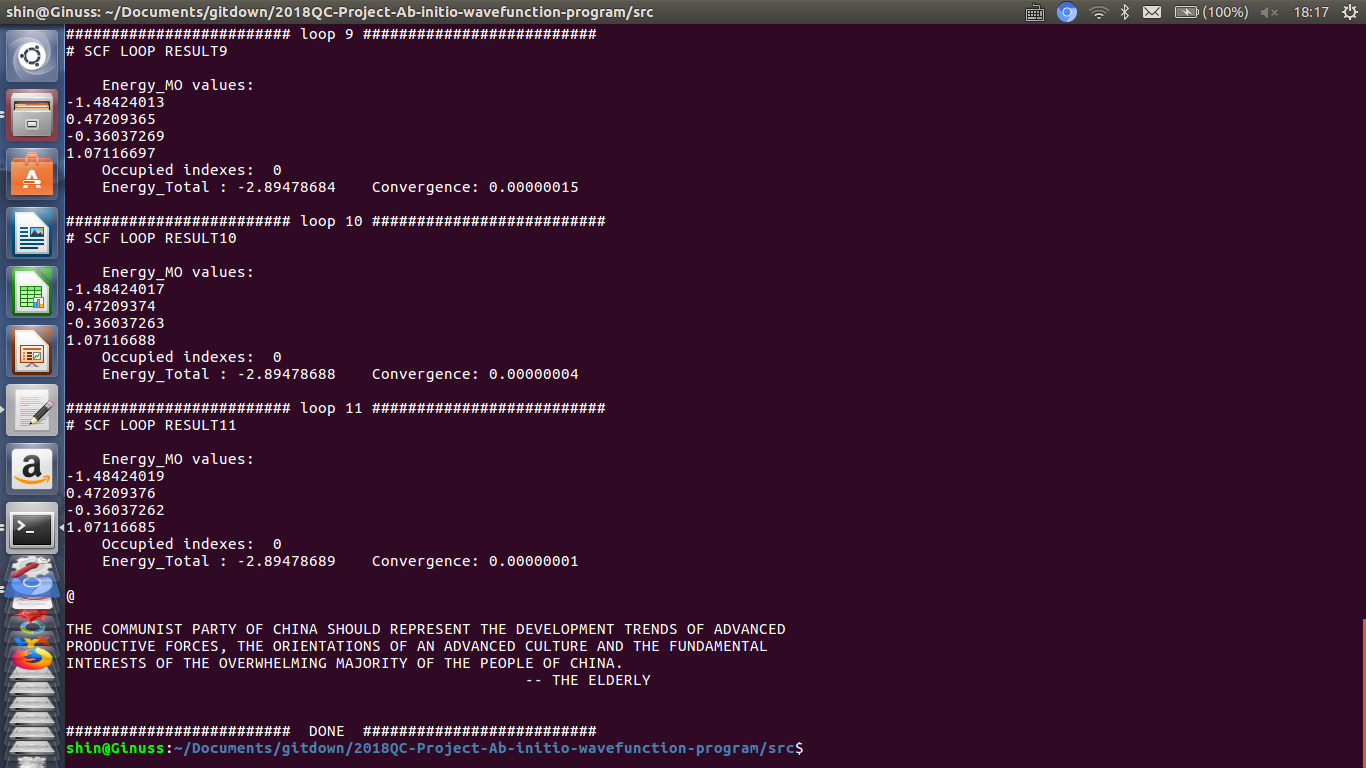
\includegraphics{./HeH+.png}
\caption{avatar}
\end{figure}


    % Add a bibliography block to the postdoc
    
    
    
    \end{document}
